\chapter{Data and Habitat Imaging
Pipeline}\label{data-and-habitat-imaging-pipeline}\label{ch:5}

This chapter describes the datasets and methods that support the
experiments carried out in this thesis. We begin by introducing the four
main patient cohorts and their role in habitat model development,
validation, and clinical application (Section 5.1). We then present the
habitat imaging pipeline (Section 5.2), our end-to-end framework for
computing tumor habitats from medical images.

\section{Patient Cohorts}\label{patient-cohorts}

\begin{figure}[htbp]
\centering
\includegraphics[width=0.95\textwidth]{fig_5_1.pdf}
\caption[Overview of patient cohorts used in this thesis]{\textbf{Overview of patient cohorts used in this thesis.}
Prospective cohorts provide multiparametric imaging (PREDICT) and
histology (POEM) for developing and validating the biologically-informed
habitat model. Retrospective cohorts (blue) provide large-scale CT
imaging with clinical outcomes for applying the habitat model and
assessing its clinical relevance. Numbers indicate patients and tumors
remaining after exclusions.}
\label{fig:5.1}
\end{figure}

This thesis is based on four main datasets of colorectal cancer patients
with liver metastases, each serving a distinct role in the development,
validation, and clinical application of CT-derived tumor habitats
(\Cref{tab:datasets}, \Cref{fig:5.1}). For the development and
biological validation of the habitat model we used two small prospective
cohorts: PREDICT (n=10 patients, 42 tumors) provides co-registered
multiparametric MRI (mpMRI) to anchor CT-derived habitats to
quantitative imaging proxies of vascularity and cellularity, while POEM
(n=6 patients, 6 tumors) provides whole-tumor histopathology for
independent validation. Two large retrospective cohorts---TCIA (n=189
patients, 389 tumors) and VHIO (n=343 patients, 1759 tumors)---provide
portal-phase CT imaging alongside clinical outcomes and are used to
apply the biologically-informed habitat model (developed in Chapter~\ref{ch:7})
and assess its prognostic value (Chapter~\ref{ch:8}). Detailed demographic and
clinical characteristics of TCIA and VHIO are provided in Chapter~\ref{ch:8}.

Chapter~\ref{ch:6} presents a broader technical study assessing the precision of
3D voxelwise radiomics features using additional retrospective data from
both liver and lung lesions. That analysis established which handcrafted
features are sufficiently robust for habitat computation and informed
the feature selection strategy used in Chapter 7. The datasets described
here---PREDICT, POEM, TCIA, and VHIO---form the foundation for the
biologically-informed habitat model and its clinical translation, which
are the central contributions of this thesis.

\begin{table}[ht]
    \centering
    \small
    \caption[Summary of datasets and their role in this thesis]{\textbf{Summary of datasets and their role in this thesis.} PREDICT provides co-registered mpMRI for biologically-informed habitat model development; POEM provides histology for independent validation. TCIA and VHIO provide large-scale CT imaging with survival outcomes for applying the habitat model and testing its prognostic value. OS: overall survival; PFS: progression-free survival; DFS: disease-free survival; mpMRI: multiparametric MRI; HE: hematoxylin and eosin.}
    \label{tab:datasets}
    
    \begin{tabularx}{\textwidth}{@{} l c c >{\raggedright\arraybackslash}X c >{\raggedright\arraybackslash}X @{}}
        \toprule
        \textbf{Dataset} & \textbf{\makecell{N\\patients}} & \textbf{\makecell{N\\tumors}} & \textbf{Imaging modalities} & \textbf{\makecell{Clinical\\outcome}} & \textbf{Primary use} \\
        \midrule
        PREDICT & 10 & 42 & CT (Portal Phase), MRI & --- & Habitat model development (mpMRI-anchored) and validation (Chapter~\ref{ch:7}) \\ \addlinespace
        POEM & 6 & 6 & CT (Portal Phase), Histology (HE) & --- & Biological validation of habitat model (Chapter~\ref{ch:7}) \\ \addlinespace
        TCIA & 189 & 389 & CT (Portal Phase) & OS, DFS & Application of habitat model and clinical outcome modeling (Chapter~\ref{ch:8}) \\ \addlinespace
        VHIO & 343 & 1759 & CT (Portal Phase) & OS, PFS & Application of habitat model and clinical outcome modeling (Chapter~\ref{ch:8}) \\
        \bottomrule
    \end{tabularx}
\end{table}

All cohorts were collected as part of ongoing studies approved by the
Vall d'Hebron University Hospital Ethics Committee: PR(AG)29/2020
(PREDICT), PR(AG)305/2024 (POEM), PR(AG)335/2018 and PR(AG)500/2023
(VHIO). Patients provided written informed consent to participate in
such studies.

\subsection{CT Image Preprocessing}\label{ct-image-preprocessing}

All CT images were acquired in the portal venous phase with
intravenous contrast, tube voltage of 100-130kV, slice thickness of
1.25-5mm and pixel size 0.7-1.1mm\textsuperscript{2}, and stored in
DICOM format (\emph{Digital Imaging and Communications in Medicine
(DICOM) Standard} \citep{DigitalImagingCommunications2025}). PREDICT and VHIO scans were retrieved from the
Vall d\textquotesingle Hebron Hospital imaging archive (Picture
Archiving and Communication System, PACS), anonymized with an
identifiable patient ID, and transferred to a password-protected VHIO
storage server. TCIA scans were downloaded from the public repository
(\url{https://www.cancerimagingarchive.net/}). POEM scans were provided
through a collaborative project with Hospital Universitari de Bellvitge
(see Section 5.1.3.) DICOM files were converted to NIfTI (Neuroimaging
Informatics Technology Initiative) format using dcm2niix \citep{liFirstStepNeuroimaging2016},

Images underwent qualitative assessment by both the author and the
group's experienced radiologists to ensure acquisition quality and
suitability for analysis. Scans were excluded if they were
non-contrast-enhanced, acquired outside the portal venous phase, did not
include the entire liver, or showed no measurable disease at baseline
(defined as liver lesions \textless1 cm in diameter or absent liver
metastases). \Cref{fig:5.1} summarizes exclusion counts for
each cohort.

For the majority of the scans, tumor segmentation was performed manually
using 3D Slicer \citep{fedorov3DSlicerImage2012}. For PREDICT and POEM, all
well-defined target lesions per patient were delineated by the group's
experienced radiologists. For VHIO cohort, a third of the tumors
(\textasciitilde600) were manually delineated by the author and
supervised by an experienced radiologist. The rest were automatically
delineated by SALSA, an automated liver tumor segmentation tool
developed in our lab during the course of this thesis, with manual
correction when needed. For TCIA, manual segmentations were performed by
radiologists as part of the original data collection \citep{simpsonPreoperativeCTSurvival2024}

Voxel resampling and intensity preprocessing were performed during
feature extraction (see Methods Section of Chapters 6 and 7), ensuring
consistent spatial resolution and intensity normalization across all
voxelwise feature maps.

\subsection{Multiparametric MRI Preprocessing (PREDICT)}\label{multiparametric-mri-preprocessing-predict}

The PREDICT cohort included contrast-enhanced CT alongside
mpMRI acquired on two scanners: a 1.5T Siemens
Avanto and a 3T GE SIGNA Pioneer. The MRI protocol included
high-resolution anatomical imaging (T2-weighted and T1-weighted),
advanced diffusion MRI with multiple b-values and echo times, variable
flip angle spoiled gradient echo (SGrE) imaging for T1 mapping, and
dynamic contrast-enhanced (DCE) MRI. Full acquisition parameters are
provided in Annex A.

MRI preprocessing was performed by MRI physicist F. Grussu, and included
denoising (MP-PCA) \citep{veraartDenoisingDiffusionMRI2016}, Gibbs unringing \citep{kellnerGibbsringingArtifactRemoval2016}, motion correction via affine coregistration \citep{ourselinReconstructing3DStructure2001}, and EPI distortion correction using reversed phase-encoding
acquisitions \citep{anderssonHowCorrectSusceptibility2003}. Anatomical images underwent N4
bias field correction based on ANTs \citep{avantsSymmetricDiffeomorphicImage2008}. Tumor
segmentations were drawn manually by an experienced radiologist on the
T2-weighted scan, aided by visual inspection of all MRI contrasts.

From the preprocessed MRI data, thirteen multiparametric (mpMRI) maps
were derived using biophysical models (\Cref{tab:mpmri_maps}). Diffusion-relaxation MRI was modeled using two approaches: (1) a
two-pool system capturing tissue and vascular water contributions,
yielding apparent diffusion coefficients ($ADC_t$, $ADC_v$), corresponding to
tissue and vascular water contributions, transverse relaxation times
($T_{2t}$), vascular signal fraction ($f_v$), and tissue kurtosis excess ($K_t$);
and (2) an advanced microstructural model \citep{grussuClinicallyFeasibleLiver2025}
incorporating intra- and extracellular compartments, yielding intrinsic
diffusivity ($D_0$), volume-weighted cell size ($vCS$), intracellular
fraction ($f_{in}$), and cell density. Variable flip angle imaging provided
total longitudinal relaxation time ($T_1$). DCE MRI was fitted using a
two-compartment Tofts model \citep{toftsModelingTracerKinetics1997}, yielding the capillary
permeability constant ($K^{trans}$), plasma volume fraction
($v_p$), and extracellular-extravascular volume fraction ($v_e$). Model
fitting was performed using custom Python code available at
\url{https://github.com/fragrussu/MyRelax} and
\url{https://github.com/fragrussu/bodymritools}.

\begin{table}[ht]
    \centering
    \small
    \caption[Multiparametric MRI maps used for CT habitat development]{\textbf{Multiparametric MRI maps used for CT habitat development.} Thirteen quantitative maps were derived from diffusion-relaxation MRI, variable flip angle T1 mapping, and dynamic contrast-enhanced MRI.}
    \label{tab:mpmri_maps}
    
    \begin{tabularx}{\textwidth}{@{} l l l c >{\raggedright\arraybackslash}X @{}}
        \toprule
        \multicolumn{2}{c}{\textbf{mpMRI metric}} & \textbf{Computed from} & \textbf{Units} & \textbf{Description} \\
        \cmidrule(r){1-2}
        $ADC_t$ & Tissue ADC & Diffusion-relaxation MRI & $\mu m^2/ms$ & Apparent diffusivity of water in tissue (excluding vasculature) \\ \addlinespace
        $ADC_v$ & Vascular ADC & Diffusion-relaxation MRI & $\mu m^2/ms$ & Apparent diffusivity in vascular compartment (IVIM effect) \\ \addlinespace
        $K_t$ & Tissue kurtosis excess & Diffusion-relaxation MRI & Dim.less & Quantifies non-Gaussian diffusion due to heterogeneity or restriction \\ \addlinespace
        $f_v$ & Vascular signal fraction & Diffusion-relaxation MRI & Norm. & Signal arising from vascular compartment (IVIM) \\ \addlinespace
        $T_{2t}$ & Tissue $T_2$ & Diffusion-relaxation MRI & ms & Transverse relaxation time of tissue (excluding vasculature) \\ \addlinespace
        $D_0$ & Intrinsic diffusivity & Advanced diffusion model & $\mu m^2/ms$ & Intrinsic intracellular diffusivity \\ \addlinespace
        $vCS$ & Vol-weighted cell size & Advanced diffusion model & $\mu m$ & Average cell size weighted by cell volume \\ \addlinespace
        $f_{in}$ & Intracellular fraction & Advanced diffusion model & Norm. & Fraction of signal arising from intracellular water \\ \addlinespace
        $CD$ & Cell density & Advanced diffusion model & Cells/$mm^3$ & Estimated cell density (derived from $f_{in}$ and $vCS$) \\ \addlinespace
        $T_1$ & $T_1$ & Variable flip angle SGrE & ms & Total longitudinal relaxation time \\ \addlinespace
        $T_2^*$ & $T_2^*$ & Multiecho SGrE & ms & Effective transverse relaxation time \\ \addlinespace
        $K^{trans}$ & Capillary permeability & DCE MRI & $min^{-1}$ & Influx mass transfer rate of contrast agent \\ \addlinespace
        $v_e$ & EES volume & DCE MRI & Norm. & Volume of extracellular, extravascular space per unit tissue volume \\
        \bottomrule
    \end{tabularx}
\end{table}

We harmonized mpMRI metrics across scanners with a custom-written ComBat
\citep{fortinHarmonizationCorticalThickness2018} implementation, rescaling metrics obtained on the
1.5T system to the 3T range. Quality control ensured that all mpMRI
values were biologically plausible. For each metric, we established a
valid range based on empirical knowledge (Annex A). Voxels within this
range were included, those marginally outside (±10\%) were clipped to
the boundary, and those beyond this tolerance were excluded.



\subsection{Histopathology Workflow (POEM)}\label{histopathology-workflow-poem}

The POEM cohort (PrOspEctive Metastases Imaging) was collected as part
of a multicenter observational study led by Dr. Peter Vermeulen (GZA
Hospitals, Belgium) in collaboration with Hospital Universitari de
Bellvitge (Spain). The study aims to develop radiomic signatures of
histopathological growth patterns \citep{lataczCanMedicalImaging2021} in liver
metastases from colorectal and breast cancer using standard-of-care CT
and MRI alongside complete histopathological sampling \citep{lataczProspectiveCompleteHistopathological2024}. Our analysis focused on colorectal liver metastases from patients
treated at Hospital Universitari de Bellvitge who underwent complete
tumor resection.

The histopathology protocol was designed to preserve spatial orientation
for comparison with preoperative imaging. Surgeons applied orientation
marks to the resected specimen, allowing the pathologist to slice the
tissue in transverse (axial) planes corresponding to CT and MRI
imaging planes. Slices were cut at 0.5--1 cm thickness, photographed,
and sampled systematically. Tissue samples were formalin-fixed,
paraffin-embedded, and stained with hematoxylin and eosin (H\&E).
Whole-slide images were acquired using a 3DHISTECH Pannoramic-series
scanner, producing MRXS files.

Histological annotations of necrosis, viable cancer and fibrosis/stroma
were automatically performed using QuPath \citep{bankheadQuPathOpenSource2017}, an
open-source digital pathology platform, and supervised by an experienced
pathologist. An experienced pathologist manually delineated regions of
necrosis, fibrosis, and viable tumor on digitized whole-slide images.
These annotations provided qualitative ground truth for validating
CT-derived habitats (Chapter~\ref{ch:7}). We attempted spatial coregistration
between histology slices and corresponding CT slices but found it
impractical due to tissue deformation during resection and processing.
As a result, histology was used for qualitative biological validation
rather than voxel-by-voxel spatial comparison.

\section{Habitat Imaging Pipeline}\label{habitat-imaging-pipeline}

Habitat imaging is becoming increasingly popular in oncology as a way to
segment tumors into meaningful radiological subregions. Yet despite a
growing literature, there is no standard tool for computing habitats.
Each study implements its own custom-built codes, which are rarely
shared and in the case they are, poorly documented. Any researcher
interested in habitat imaging faces the same challenges repeatedly: how
to preprocess voxelwise features, how to choose the clustering
algorithm, how to ensure habitat labels are across patients are
consistent so that ``Habitat 1'' means the same thing in every case,
etc.

These are not trivial implementation choices. A pipeline that ignores
voxel spacing differences will produce habitats that reflect acquistion
parameters rather than biology. A pipeline that clusters all tumors
together may dilute tumor-specific heterogeneity into noise. The
experiments carried out in Chapter~\ref{ch:6} made these challenges concrete for
us. Computing habitats for the precision analysis requires solvign each
of these problems from scratch, and the solutions were tied to the
specific dataset and analysis.

To enable the work in Chapters 7 and 8, and to support future research,
we developed a modular, documented pipeline that addresses these issues
systematically. The pipeline is image-modality agnostic, being
applicable to any voxelwise imaging data (CT, MRI, PET, etc.) and
works with both 2D and 3D data. It also includes key design choices as
configurable parameters rather than hardcoded assumptions. We are
currently preparing the pipeline for public release as an open-source
tool, available at
https://github.com/radiomicsgroup/imaging-habitats-pipeline. We share it
with the hope that it saves other researchers the substantial time and
effort required to build habitat imaging workflows from scratch, and
that it helps standardize methods across studies to improve
reproducibility and comparability in the field.

\subsection{Pipeline Overview}\label{pipeline-overview}

The pipeline consists of three modules: Preprocessing, Clustering, and
Analysis (\Cref{fig:5.2}):

\begin{itemize}
\item
  \textbf{Preprocessing} takes voxelwise feature maps (e.g., Kurtosis,
  ADC, Coarseness) as 3D NIfTI files, removes background voxels,
  enforces consistent array shapes across maps, and applies feature
  scaling. The output is a 4D NIfTI volume per tumor (dimensions: x, y,
  z, features), with both scaled and unscaled versions preserved for
  transparency. Background voxels are automatically detected and masked
  out, and all feature maps are checked for spatial alignment.
\item
  \textbf{Clustering} takes the preprocessed 4D volumes and assigns each
  voxel to a habitat. The module supports multiple algorithms (Gaussian
  Mixture Models, K-means, Bayesian GMM, HDBSCAN) and allows the number
  of clusters to be set manually or selected via data-driven criteria
  (BIC, silhouette score). Cluster labels are integers starting at 1;
  background is reserved as 0.
\item
  \textbf{Analysis} computes habitat-derived metrics (described in
  Section 5.2.4) and exports summary statistics as CSV files for
  downstream analysis.
\end{itemize}

\begin{figure}[t!]
\centering
\includegraphics[width=0.95\textwidth]{fig_5_2.pdf}
\caption[Habitat imaging pipeline overview]{\textbf{Habitat imaging pipeline overview.}
The pipeline consists of three modules. Preprocessing removes background
voxels, applies optional log transformation, and performs standard
scaling, outputting a 4D NIfTI volume per tumor. Clustering assigns
voxels to habitats using GMM, K-means, Bayesian GMM, or HDBSCAN, with
automatic or manual selection of cluster number. Three clustering scopes
are available: single-tumor, pooled, or hybrid (Figure~\ref{fig:5.3}). Analysis computes
habitat-derived metrics (proportions, entropy, rim/core statistics) and
exports summary tables.}
\label{fig:5.2}
\end{figure}



The pipeline is implemented in Python and can be run from the command
line. All random seeds are exposed for reproducibility, and outputs are
organized by experiment name to support version control.

\subsection{Key Implementation Choices}\label{key-implementation-choices}

\textbf{Voxel resampling.} Texture features describe spatial
relationships between neighboring voxels, which means their values
depend on voxel dimensions. A feature computed on a 0.7×0.7×1.0 mm grid
is not directly comparable to the same feature computed on a 0.9×0.9×2.5
mm grid. For cross-tumor comparisons to be meaningful, input images
should be resampled to a common isotropic resolution before feature
extraction. The pipeline itself does not yet perform resampling---it
expects preprocessed inputs---but users working with heterogeneous
acquisitions should resample upstream since results may reflect
acquisition differences rather than biology.

\textbf{Feature scaling.} Clustering algorithms are sensitive to feature
magnitudes. If one feature ranges from 0 to 1 and another from 0 to
10,000, the latter will dominate distance calculations regardless of its
biological relevance. We apply standard scaling (zero mean, unit
variance) to all features before clustering. The scaler can be fit per
tumor, per patient, or across the full cohort, depending on the analysis
goal. For the studies in this thesis, we fit a single scaler across all
voxels being processed, ensuring that habitat definitions are comparable
across tumors.

\textbf{Log transformation.} Some imaging metrics span several orders of
magnitude and exhibit strong right skew---ADC values, T1 relaxation
times, and permeability coefficients are common examples. Clustering
such features in their raw form can produce habitats driven by outliers
rather than typical tissue properties. We assess each
feature\textquotesingle s distribution (skewness, dynamic range,
coefficient of variation) and apply log transformation where
appropriate, excluding bounded fractions (e.g., volume fractions
constrained to {[}0,1{]}) to preserve their probabilistic
interpretation. This is not a universal preprocessing step; it is a
decision that must be made feature by feature, with the goal of
presenting the clustering algorithm with distributions that reflect
meaningful biological variation rather than measurement artifacts.

\textbf{Clustering algorithm and number of clusters.} The pipeline
supports multiple clustering algorithms: Gaussian Mixture Models (GMM),
K-means, and HDBSCAN. GMM is our default because it provides
probabilistic (soft) assignments that better capture gradual transitions
between tumor phenotypes---biologically plausible given partial volume
effects and mixed tissue interfaces. However, users may prefer hard
assignments or density-based clustering depending on their application.
The number of clusters can be specified manually or determined
automatically using different criteria such as the Bayesian Information
Criterion (BIC) or the Silhouette Score.

\textbf{Clustering Scope:} A critical design choice is whether to
cluster each tumor individually or pool all tumors together. The
pipeline supports three modes (\Cref{fig:5.3}):

\begin{figure}[t!]
\centering
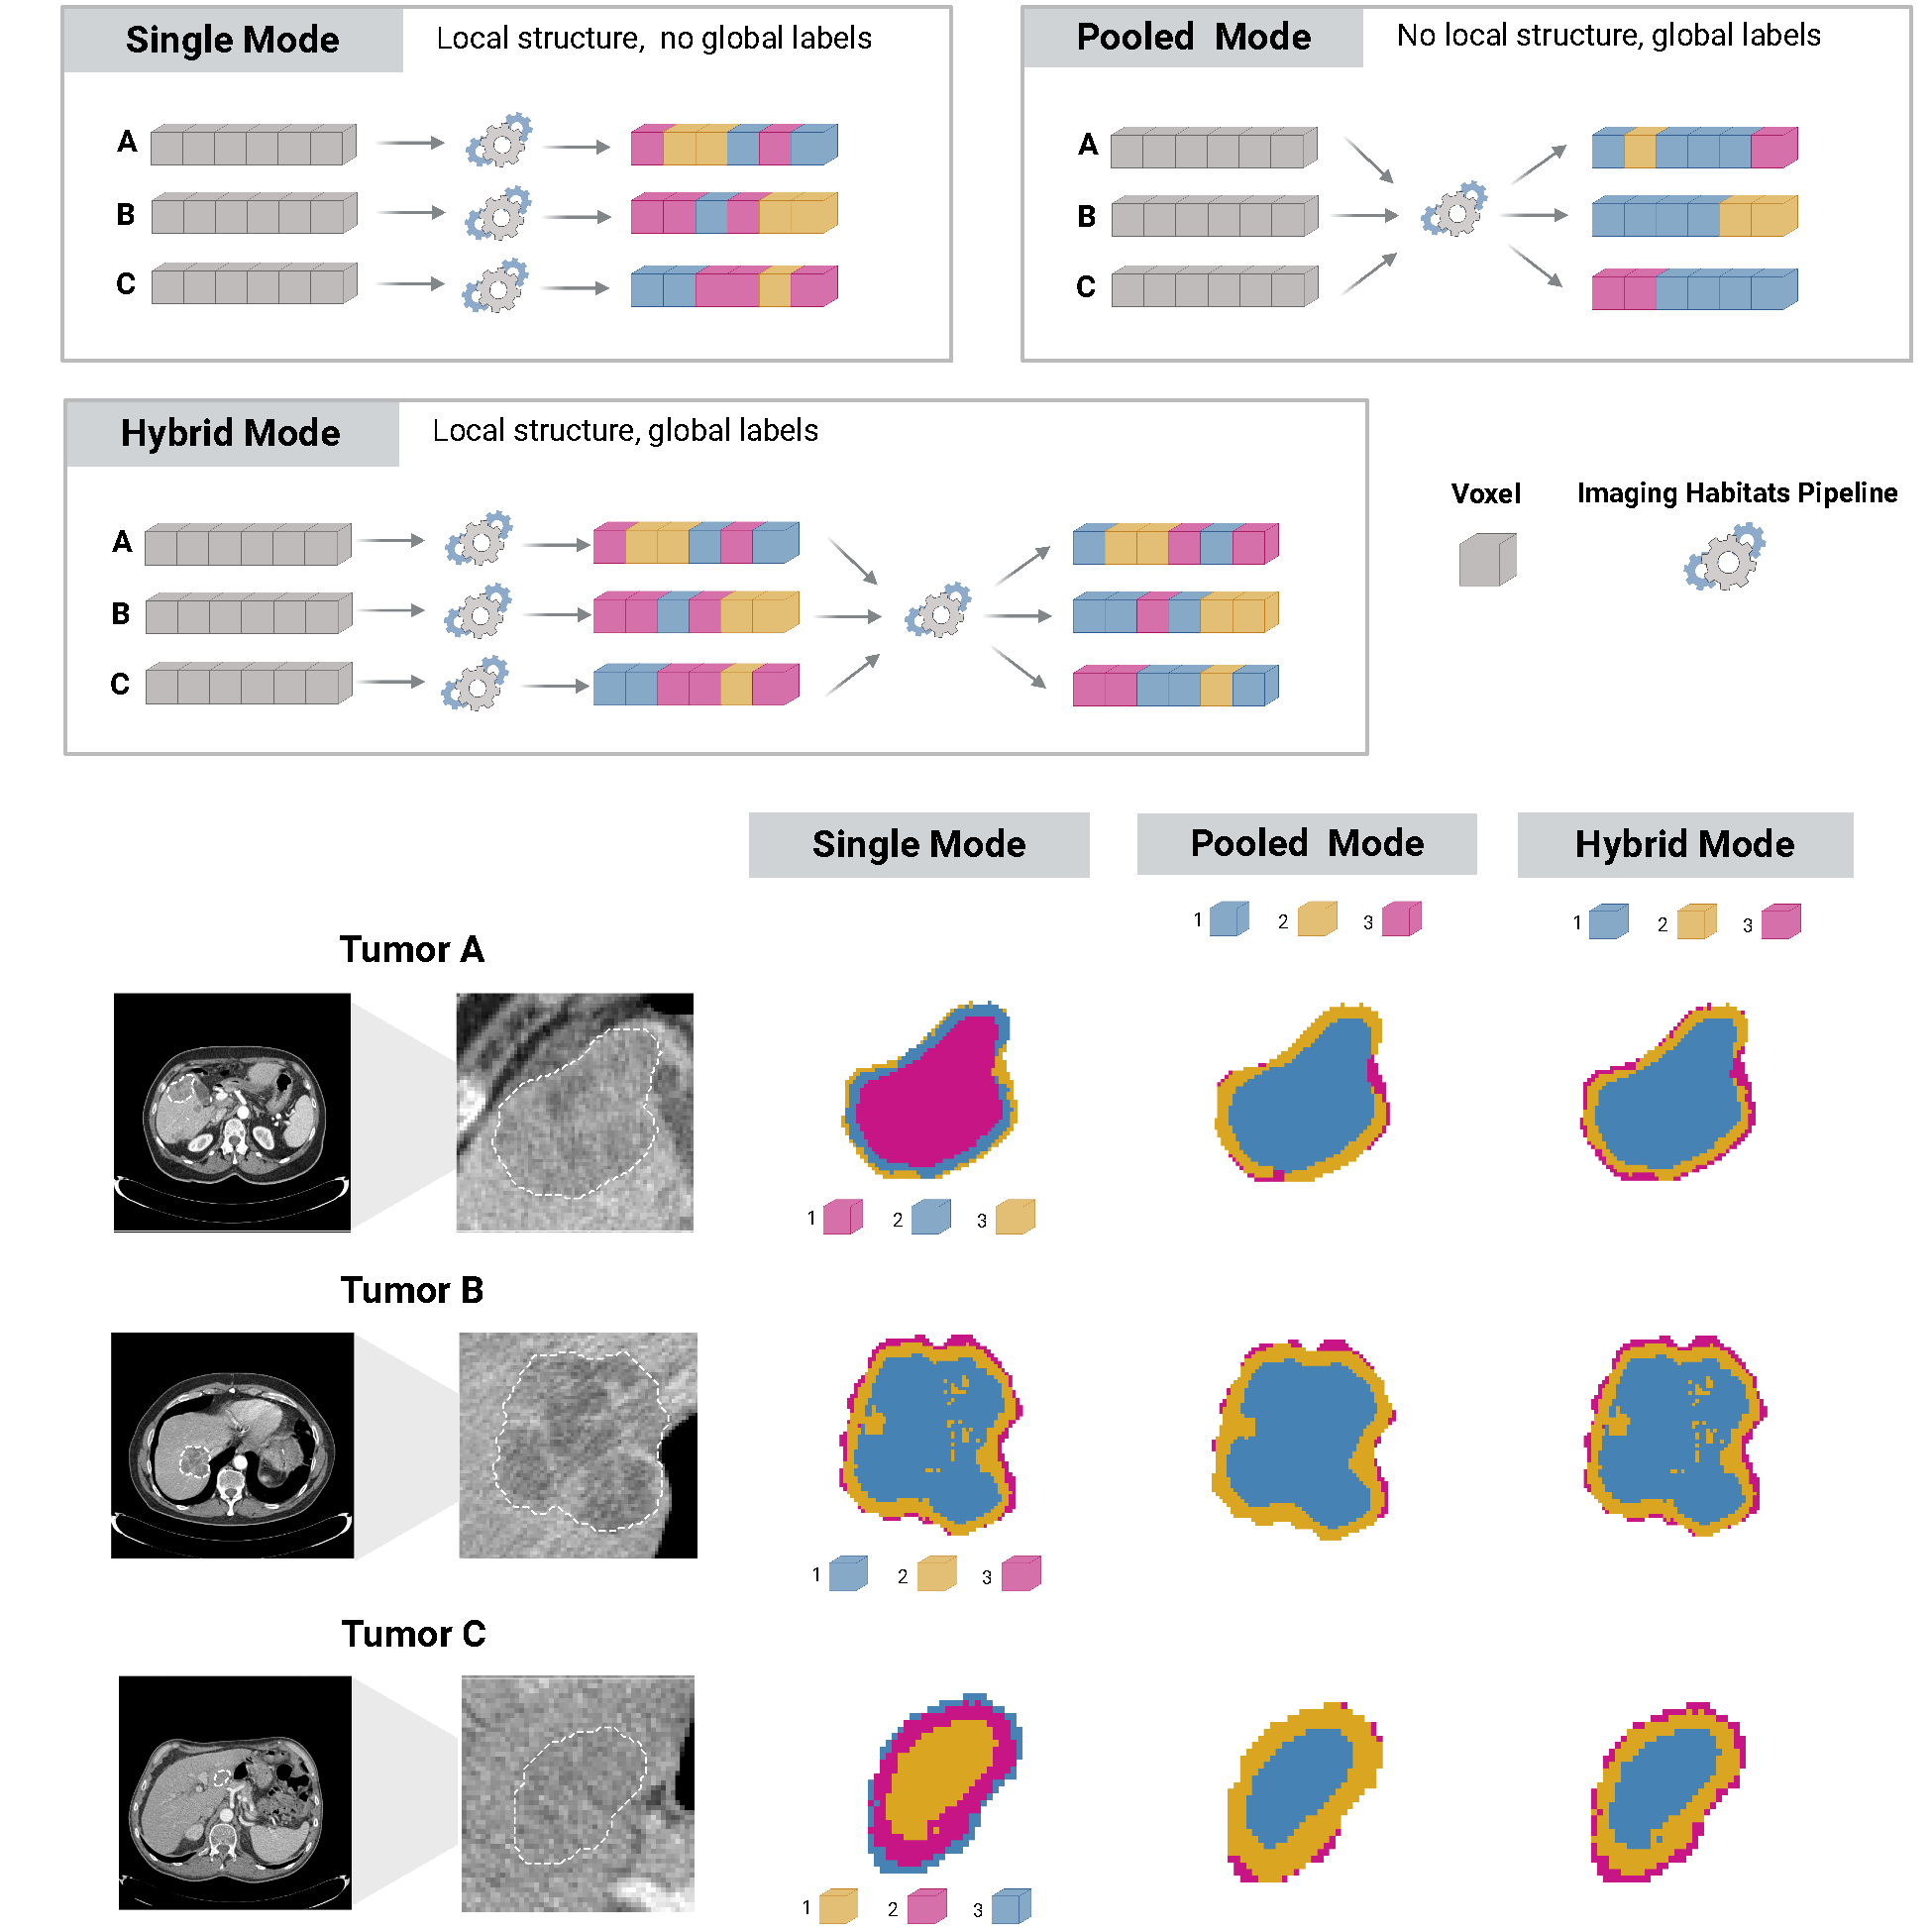
\includegraphics[width=0.9\textwidth]{fig_5_3.pdf}
\caption[Clustering scope: single-tumor, pooled, and hybrid modes]{\textbf{Clustering scope: single-tumor, pooled, and hybrid modes.}
\textbf{(A)} Single-tumor mode. Each tumor is clustered independently.
Labels are arbitrary and not comparable across tumors. \textbf{(B)}
Pooled mode. All voxels are clustered together, producing globally
consistent labels. However, local heterogeneity may be diluted.
\textbf{(C)} Hybrid mode. Tumors are first clustered locally, then local
cluster centroids are pooled and meta-clustered to define global
prototypes. Each local cluster is mapped to its nearest prototype,
yielding consistent labels while preserving local structure.}
\label{fig:5.3}
\end{figure}

\emph{Single-tumor mode} clusters each tumor independently. This
preserves local heterogeneity patterns but produces arbitrary label
IDs---"Cluster 1" in Tumor A might represent necrosis, while "Cluster 1"
in Tumor B might represent highly perfused tissue. Cross-patient
comparisons require post-hoc label alignment.

\emph{Pooled mode} stacks all voxels from all tumors and clusters them
in a single run. Labels are globally consistent by construction: every
voxel in the cohort is assigned to one of K shared habitats. However,
pooling can dilute tumor-specific patterns. If one tumor is
predominantly necrotic and another highly vascular, the algorithm may
find "average" habitats that represent neither tumor well. Inter-tumor
variability in baseline intensities can dominate the clustering,
obscuring biologically meaningful intra-tumor structure.

\emph{Hybrid mode} combines both strategies through a two-level
approach:

\begin{enumerate}
\def\labelenumi{\arabic{enumi}.}
\item
  \emph{Local clustering}: Each tumor is clustered independently (as in
  single-tumor mode), preserving fine-grained heterogeneity.
\item
  \emph{Centroid extraction}: The centroid (mean feature vector) of each
  local cluster is computed, producing a compact representation of each
  tumor\textquotesingle s habitat structure.
\item
  \emph{Meta-clustering}: All centroids from all tumors are pooled and
  clustered again. The resulting cluster centers define \emph{global
  prototypes}---canonical imaging phenotypes that recur across the
  cohort.
\item
  \emph{Label assignment}: Each local cluster is mapped to its nearest
  global prototype, producing globally consistent habitat labels while
  respecting local tumor structure.
\end{enumerate}

\textbf{Label harmonization.} Regardless of clustering mode, local
cluster labels are arbitrary---determined by algorithm initialization,
not biology. The pipeline provides an optional harmonization step that
reorders labels based on a biologically meaningful reference feature
(e.g., median Hounsfield units). After harmonization, Habitat 1
consistently represents the lowest-intensity phenotype across all
tumors, Habitat K the highest. This can be applied to any mode.



\subsection{Habitat-Derived Quantitative Metrics}\label{habitat-derived-quantitative-metrics}

Once habitats are defined, the pipeline computes metrics that summarize
tumor composition and heterogeneity. For each tumor, we calculate:

\begin{itemize}
\item
  \textbf{Habitat proportions}: The fraction of tumor volume assigned to
  each habitat. A tumor might be 60\% Habitat 1, 30\% Habitat 2, and
  10\% Habitat 3. Differences in these proportions across patients may
  correlate with clinical outcomes.
\item
  \textbf{Shannon entropy}: A single number quantifying habitat
  diversity, calculated as
\end{itemize}

\begin{quote}
\[H(p) = - \sum_{i = 1}^{K}{p_{i}\log_{2}p_{i}}\]

\(p_{i}\,\)is the proportion of habitat \emph{i}. Entropy is maximized
when habitats are equally distributed (high heterogeneity) and minimized
when one habitat dominates (low heterogeneity).
\end{quote}

The pipeline outputs clustered NIfTI files, allowing users to compute
additional metrics as needed. In our studies of liver metastases
(Chapters 7 and 8), we observed that tumors often exhibit a viable rim
surrounding a necrotic core---a spatial pattern with potential
prognostic relevance. To capture this, we extended the metrics to
separate tumor subregions:

\begin{itemize}
\item
  \textbf{Rim}: The outer shell within a specified distance from the
  tumor boundary, computed using signed distance transforms.
\item
  \textbf{Core}: The interior region remaining after excluding the rim.
\end{itemize}

The rim thickness is a user-defined parameter. In this thesis, we use a
default of 2 mm based on biological considerations: tumor cells cannot
survive more than approximately 2 mm from a blood vessel due to the
diffusion limits of oxygen and nutrients \citep{thngPerfusionMagneticResonance2010}. This distance
defines the maximum viable thickness of tissue without direct vascular
supply, and is the rationale underlying anti-angiogenic therapies that
target tumor neovascularization. For each subregion, we compute habitat
proportions and entropy separately. High rim entropy, for example, may
reflect an active tumor-host interface with mixed viable tumor and
vascular remodeling, while low core entropy may indicate uniform
necrosis. These spatially-resolved metrics are used as imaging
biomarkers in the clinical analyses of Chapter 8.

